\documentclass[a4j,9pt,twocolumn]{paper}
\usepackage[dvipdfmx]{graphicx}
\usepackage{amsmath}
\usepackage[hang,small,bf]{caption}
\usepackage[subrefformat=parens]{subcaption}
\captionsetup{compatibility=false}

\usepackage[varg]{txfonts}

%%% \begin{document}の前に,各エントリーを記述する

\title{タクシーの運転支援システム構築に関する研究}	% 論文のタイトル
\author{広本 将基}		% 著者
\studentid{29C15073}	% 学籍番号
\lab{潮}		% 研究室名

% 英語なら以下2行を定義
%\englishtitle
%\jptitle{日本語の題名}  % 日本語のタイトル

\begin{document}
\absttitle		% 表題の出力

\section{緒論}
\par
流しのタクシーが効率よく乗客をのせるための支援システムの開発は,運転手の待遇改善につながる重要な課題である.
本論文では,過去の乗車データと現在の流しのタクシーの分布から,モデル予測制御を応用して最適な進行方向を決定する方法を提案する.

\section{提案モデル}
\par
対象領域を$N$個の部分領域(セル)に分割する.
時刻$k$のときのセル$i$($i = 1, 2, \ldots, N$)での空車数を$x_i(k)$とおく.
時間区間$[k,\ k+1)$の間に,領域$i$で実車になるタクシー数を$s_i(k)$,空車になるタクシー数を$e_i(k)$とおく.
入力として,時間区間$[k,\ k+1)$の間にセル$i$からセル$j$へ移動する空車数を$u_{i, j}(k)$とおく.
このとき,各セルの空車数のダイナミクスは,
\begin{align}
 x_i(k+1) = x_i(k)-s_i(k)+e_i(k)+\sum_{j=1}^{N}\bigg(u_{j,i}(k)-u_{i,j}(k) \bigg) \label{eq:x}
\end{align}
となる.

\par
$d_i(k)$を時間区間$[k,\ k+1)$の間にセル$i$で乗車できなかった客数とおくと,
\begin{align}
 d_i(k+1) = d_i(k)-s_i(k)+p_i(k)
\end{align}
である.
ただし,$p_i(k)$は時間区間$[k,\ k+1)$の間で発生する新たな乗客数で,過去の乗車データから予測される.
時間区間$[k,\ k+1)$に間に空車になるタクシー数$e_i(k)$は
\begin{align}
 e_i(k)=\beta_{i}r(k) \label{eq:e}
\end{align}
とする.
ただし,$r(k)$は時刻$k$のときの実車の総数で,$\beta_{i}$は過去のデータから推定される実車全体の中でセル$i$で空車になる割合である.
実車の総数$r(k)$は,式(\ref{eq:e})を用いると
\begin{align}
 r(k+1) = \bigg(1-\sum_{i=1}^{N}\beta_i\bigg)r(k)+\sum_{i=1}^{N}s_i(k) \label{eq:r}
\end{align}
と表される.
ここで,入力に関する制約として,各セル$i$について
\begin{align}
 x_i(k)=\sum_{j=1}^{N}u_{i,j}(k) \label{eq:input}
\end{align}
を与える.
このように移動する空車数を定めると,式(\ref{eq:x}),\ (\ref{eq:e}),\ (\ref{eq:input})からシステムダイナミクスは
\begin{align}
 x_i(k+1)=\beta_i r(k)-s_i(k)+\sum_{j=1}^{N} u_{j,i}(k) \label{eq:simple_system}
\end{align}
となる.
ここで,式(\ref{eq:r}),\ (\ref{eq:input}),\ (\ref{eq:simple_system})からタクシーの総数は変化しないことを示せるので,タクシーの総数を$L$とおくと
\begin{align}
 r(k)= L-\sum_{i=1}^{N}x_i(k) \label{eq:r_new}
\end{align}
とおける.
さらに,時間単位で隣接するセルにしか移動できないと仮定する.このとき,
セル$i$に隣接しないセル$\ell$については
\begin{align}
 u_{i, \ell}(k)=0 \qquad  \forall k \label{eq:u_seiyaku}
\end{align}
となる.
ここで,時間区間$[k,\ k+1)$の間で実車になる台数$s_i(k)$については
\begin{align}
 s_i(k)=\left\{
\begin{array}{ll}
 \alpha_i d_i(k) & \mbox{if }h_i(k) \geq 0 \\
h_i(k)+\alpha_i d_i(k) & \mbox{otherwise}
\end{array}\right. \label{eq:s2}
\end{align}
と表すことができる.
ただし,$\alpha_i$は領域$i$において過去のデータから推定されるタクシーに乗車できる乗客の割合である.
また,
% \begin{align}
%  h_i(k)=\beta_i \bigg( L-\sum_{j=1}^{N}x_j(k)\bigg) +\sum_{j=1}^{N}u_{j,i}(k) -\alpha_i d_i(k) \label{eq:h}
% \end{align}
\begin{align}
 h_i(k)=\beta_i r(k) +\sum_{j=1}^{N}u_{j,i}(k) -\alpha_i d_i(k) \label{eq:h}
\end{align}
である.
ここで,式(\ref{eq:s2})は条件付きの式になっているため,ソルバーで扱える形に変形する必要がある.
そのため,以下の論理変数$\delta_i(k) \in \{ 0,\ 1\}$を導入する.
\begin{align}
 \delta_i(k)=
\left\{ \begin{array}{ll}
1 & \mbox{if }h_i(k)\geq 0 \\
0 & \mbox{otherwise}
\end{array} \right. \label{eq:delta}
\end{align}
このとき,制約条件式(\ref{eq:delta})は次の不等式制約条件になる.
\begin{align}
 h^{inf}_{i}(1-\delta_i(k))\leq h_i(k) \leq h^{sup}_{i} \delta_i(k)+(\delta_i(k) -1) \epsilon \label{eq:delta_new}
\end{align}
ただし,$\epsilon$は十分に小さく,$h^{inf}_{i}\leq h_i(k)\leq h^{sup}_{i}$である.
論理変数を用いることで式(\ref{eq:s2})は以下の制約条件に変形される.
\begin{align}
& s_i(k) = z_i(k)+h_i(k)+\alpha_i d_i(k)\\
& -h^{sup}_{i} \delta_i(k) \leq z_i(k) \leq -h^{inf}_{i} \delta_i(k)\\
& -h_i(k)+h^{inf}_i (1-\delta_i(k)) \leq z_i(k) \leq -h_i(k)+h^{sup}_i (1-\delta_i(k))
\end{align}
これらの式を制約条件とする最適化問題は混合性数計画問題である.

\par
以上の制約式のもとで,時刻$t$において次の目的関数を最小化する有限区間最適化問題を考えた.
\begin{align}
\mbox{minimize }J_t=\sum_{i=1}^{N}d_i(t+T) \label{eq:ob_function}
\end{align}
ただし,$T$は正の整数である.

\section{実装結果}
\begin{figure}[h]
  \begin{minipage}[b]{0.5\linewidth}
    \centering
    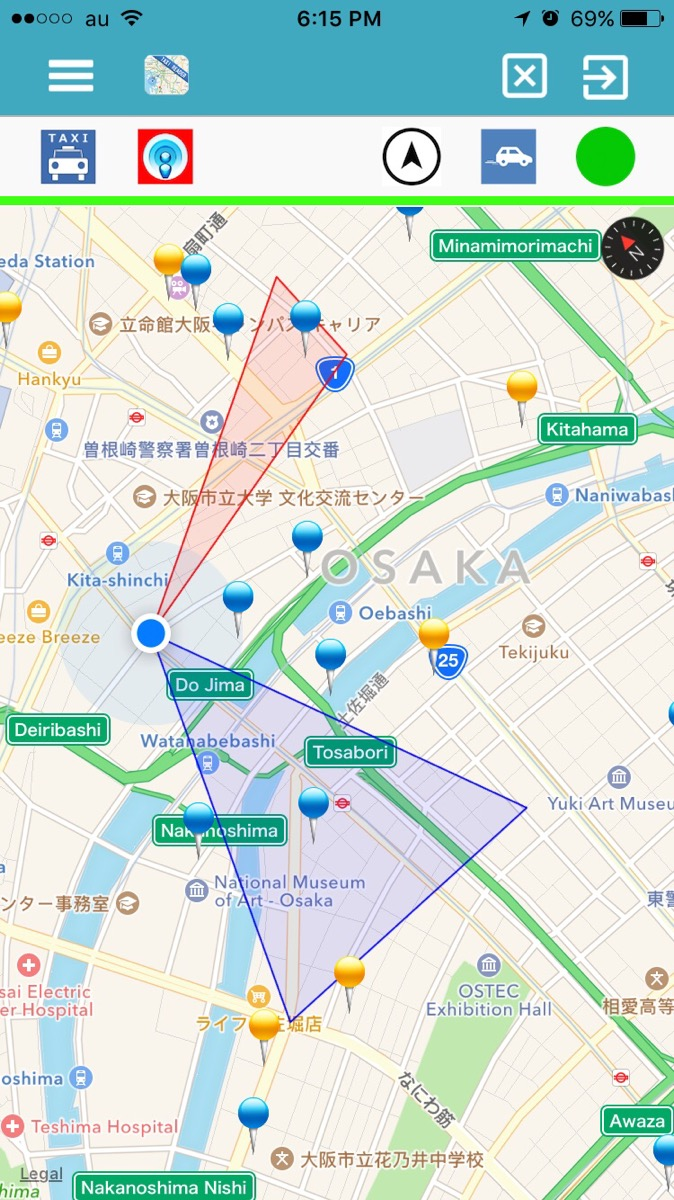
\includegraphics[keepaspectratio, width=22mm]{Graphics/201603311815.jpg}
    \subcaption{2016年3月31日18時15分}\label{fig:fig1-1}
  \end{minipage}
  \begin{minipage}[b]{0.5\linewidth}
    \centering
    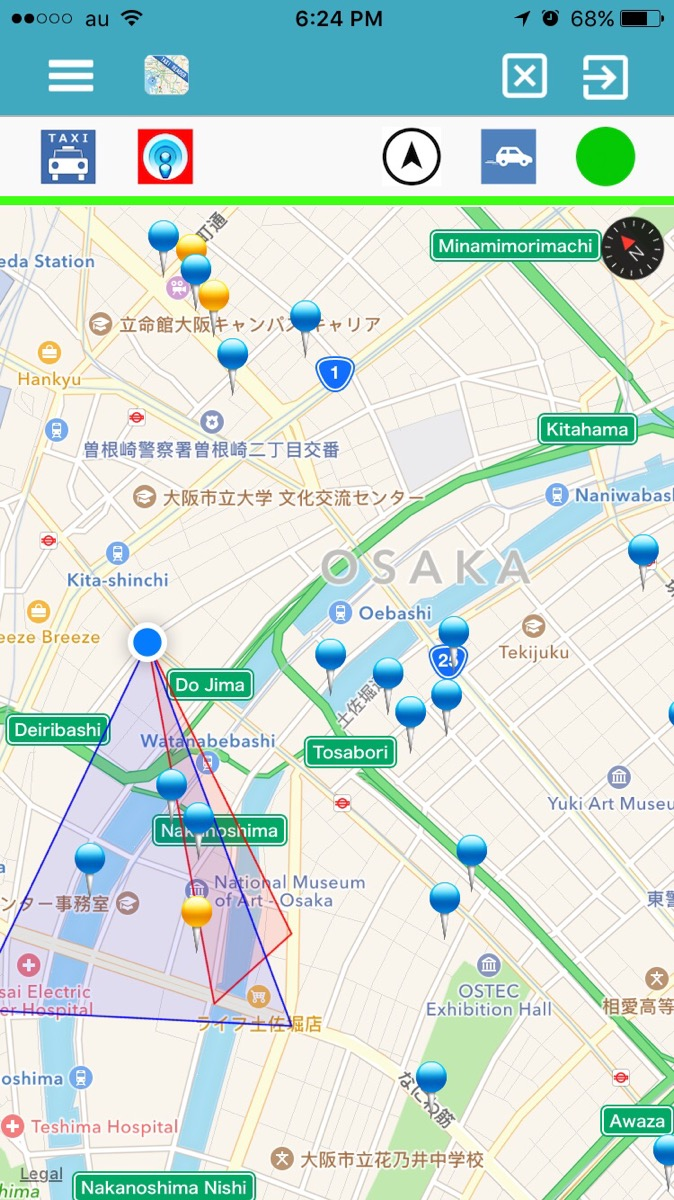
\includegraphics[keepaspectratio, width=22mm]{Graphics/201603311824.jpg}
    \subcaption{2016年3月31日18時24分}\label{fig:fig1-2}
  \end{minipage}
  \caption{最適方向の時間的変化}\label{fig:fig1}
\end{figure}
図\ref{fig:fig1}は大阪駅から難波駅あたりまでを対象範囲としたときの実装結果である.1辺の長さ2kmの正方形のセルを使って$N=24$セルに分割した.
2分を1時間単位として,$T=2$でモデル予測制御により最適移動分布を計算した.
青色が示す方向は最適移動分布の最大値を示す方向である.
赤色が示す方向は周囲で乗車箇所が最も多い方向,すなわち,貪欲な方向である.
この結果から,最適な方向と貪欲な方向が必ずしも一致しないことがわかる.

%\bibliographystyle{junsrt}
%\bibliography{refs}
% \begin{thebibliography}{1}
% \bibitem{1}F. Miao, et al., “Taxi Dispatch with Real-Time Sensing Data in Metropolitan Areas- a Receding Horizon Control Approach.”,  Proceedings of ICCPS 2015, pp. 100-109, 2015
% \end{thebibliography}
\newpage
\pagebreak
\end{document}
